\chapter{Experimentos.}\label{cap.experimentos}
\hspace{1cm} En este cap\'itulo se van a comentar las distintas pruebas realizadas tanto con el drone real como en la simulaci\'on, las cuales validan cada fase del proyecto y la soluci\'on final. Tambi\'en estas pruebas han servido para depurar mientras se desarrollaba. 

\hspace{1cm} Antes de comenzar, comentar diferencias importantes que hay entre trabajar en el entorno simulado y en el real. Primero, en el entorno simulado los colores puros ideales y mas f\'aciles de detectar, sin embargo en el entorno real debido a luces y sombras un color puede verse mas o menos n\'itido, adem\'as de ser mas dif\'icil aislarlo del resto. Tambi\'en las velocidades a aplicar sobre uno y otro son distintas, pues en el entorno simulado se le puede dar una mayor velocidad que trabajara sin problemas, sin embargo en el real una velocidad alta y un movimiento brusco puede llevar a desestabilizarlo. 

\hspace{1cm} Por otra parte, en el drone real se daba el factor de la bater\'ia, en funci\'on de la carga que tuviera esta aterrizaba con mas o menos fuerza y realizaba movimientos mas o menos fluidos. A partir del 30\% de bater\'ia no permit\'ia al drone realizar todos los movimientos, y en algunas ocasiones perd\'ia altura, aunque despues volv\'ia a ganarla. 

\hspace{1cm} Para organizar las distintas pruebas,  se va a hablar sobre la parte de percepci\'on. Tras esto se comentara por separado cada una de las partes del algoritmo (despegue, b\'usqueda y aterrizaje), para terminar con una ejecuci\'on t\'ipica del algoritmo completo.

\section{Percepci\'on. }

\hspace{1cm} Para las pruebas de esta secci\'on, hay que tener en cuenta el objeto a detectar. Como ya se ha dicho anteriormente, este trata de un cuadrado con cuatro cuadrados dentro, dos de color naranja, y otros dos de color azul (trabajando con el drone real) o verde(si se trabajaba en un entorno simulado. 

\hspace{1cm} Los primeros test se realizaban en el entorno simulado, al principio detectando ambos colores y viendo que se trataba de 4 objetos distintos. Despu\'es se comenzaron los test con el algoritmo final, viendo que los cuatro cuadrados formaban una cruceta y detectaba esta en la \'imagen, para as\'i poder centrarse. Dependiendo de los distintos estados del algor\'itmo, cuando ve\'ia una parte de la baliza la detectaba y marcaba como posible objeto, en caso de tratarse de la baliza completa la marcaba como tal. 

\begin{figure}[H]
 \centering
  \subfloat[Percepci\'on posible objeto]{
   \label{f:Posible objeto}
    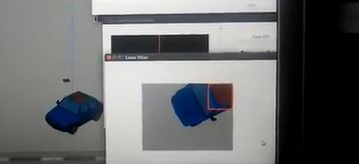
\includegraphics[width=0.4\textwidth]{imgs/perception1.jpg}}
  \subfloat[Detecta objeto]{
   \label{f: Deteca objeto}
    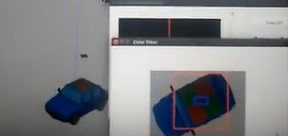
\includegraphics[width=0.4\textwidth]{imgs/perception2.jpg}} 
 \caption{Drone detectando objeto.}
 \label{f:Drone detecta objeto. }
\end{figure} 

\hspace{1cm} Una vez se realizaron estos con \'exito, pasaron a realizarse las pruebas con el drone real. Las primeras pruebas eran con el drone quieto y situando las balizas en distintas posiciones y viendo que las detectaba. Tras esto con el drone volando se hicieron pruebas, viendo que cuando se situaba la baliza debajo de este era capaz de detectarla. 

\begin{figure}[H]
	\centering
		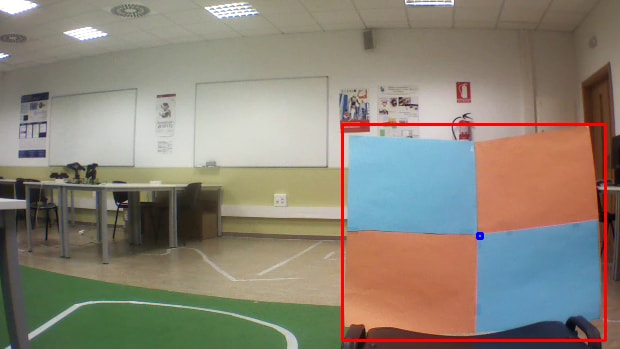
\includegraphics[width=0.55\textwidth]{imgs/k_beacon21.jpg}
		\caption{Detectando baliza real.}
	\label{fig:Detectando baliza real.}
\end{figure}

\section{Despegue.}

\hspace{1cm} Las primeras pruebas del despegue sobre el simulador fueron las mas sencillas. Esto se debe a que se trata de un entorno ideal en el cual el drone no tiene deriva ni se dan otros factores externos. Las pruebas consist\'ian en despegar el drone y que este se centrara sobre la baliza, aunque tambi\'en se prob\'o a despegar el drone sobre el coche con la baliza y mover el coche para ver que el drone le iba siguiendo. Esta parte se decidi\'o implementar porque el drone ten\'ia una deriva que le llevaba a desplazarse hacia atr\'as cuando ten\'ia que estar en el sitio. Cuando se hicieron las primeras pruebas de esto, se vi\'o que el drone siempre despegaba en esta direcci\'on y hab\'ia un dos segundos en los que no se pueden controlar sus movimientos, por tanto hab\'ia que contar con este desplazamiento.
\begin{figure}[H]
	\centering
		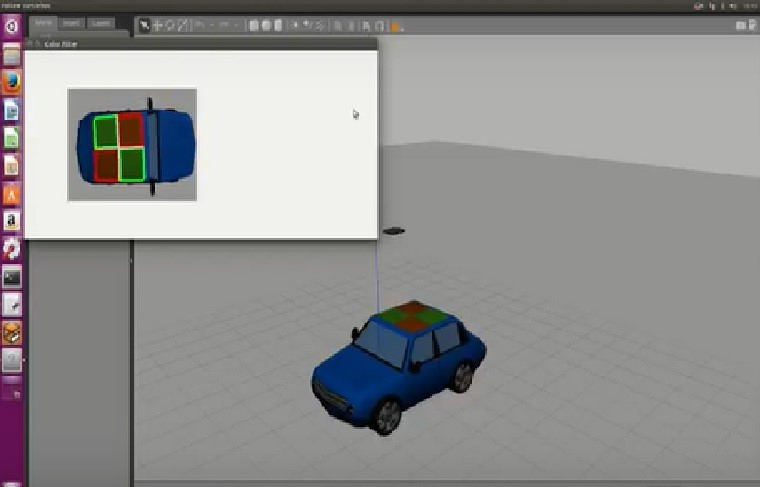
\includegraphics[width=0.4\textwidth]{imgs/TakeOff.jpg}
	\label{fig:Despegue sobre la baliza del coche.}
\end{figure}


\hspace{1cm} Para la realizaci\'on de este experimento situ\'abamos la baliza real sobre el suelo y el drone sobre esta, y as\'i al despegar ten\'ia un punto sobre el que centrarse. 

\begin{figure}[H]
 \centering
  \subfloat[Despegue vista baliza]{
   \label{f:Vista baliza}
    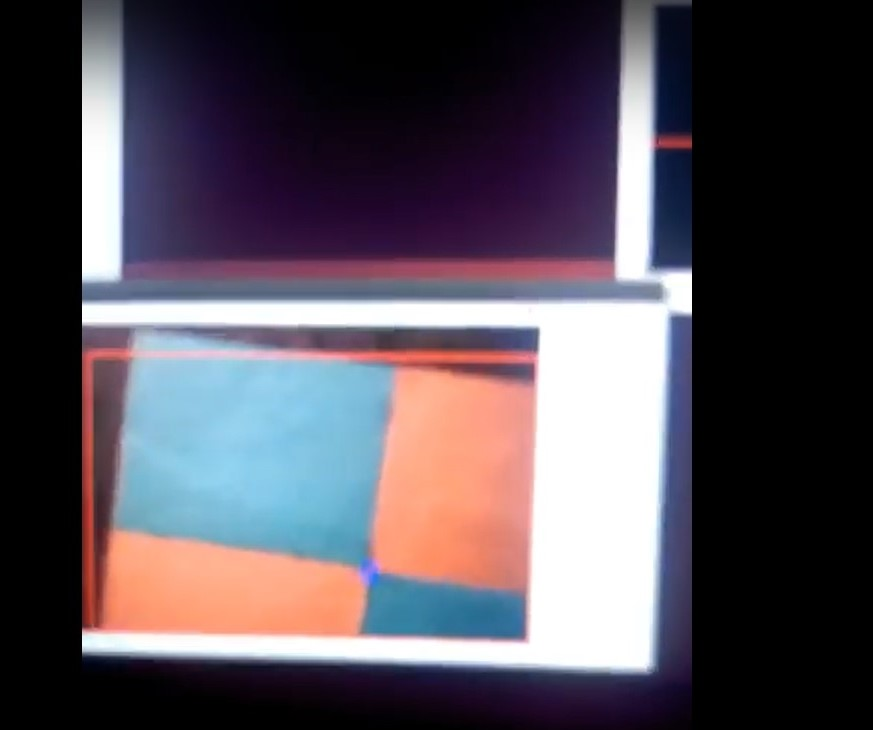
\includegraphics[width=0.4\textwidth]{imgs/takeoff_baliza.jpg}}
  \subfloat[Despegue vista drone]{
   \label{f:Drone}
    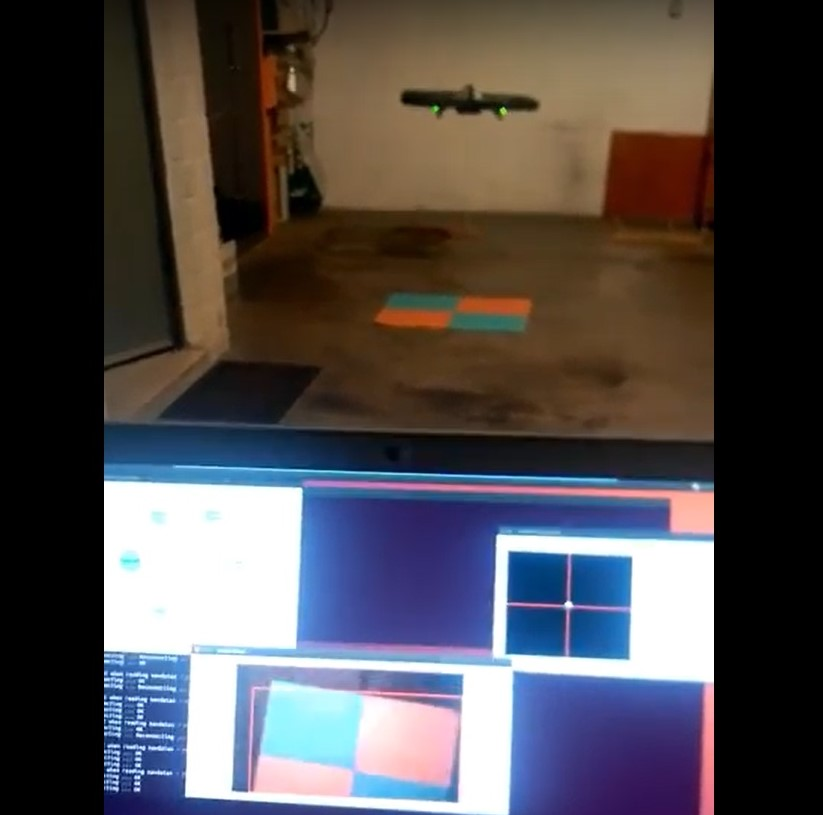
\includegraphics[width=0.4\textwidth]{imgs/takeoff_baliza2.jpg}}
 \caption{Despegue}
 \label{f:Test Despegue}
\end{figure}

Para la realizaci\'on del algoritmo, el periodo de despegue se controla por tiempo, dejando 10 segundos para este. 
En el siguiente enlace esta el video con el despegue real del drone:\\
\underline{\url{https://www.youtube.com/watch?time_continue=26&v=HVGSlbA1tq4}}

\section{B\'usqueda. } Para la realizaci\'on de \'esta parte del algoritmo, como ya he comentado anteriormente, el drone va movi\'endose en espiral hasta encontrar la baliza, para ya centrarse sobre esta. Al principio de los experimentos, el drone se situaba cerca de la baliza para empezar su desplazamiento y que al encontrar la baliza se centrara. Una vez esto funcionaba, se probaba a poner el drone m\'as lejos de \'esta para que en la primera vuelta de la espiral no encontrara ning\'un objeto de inter\'es, pero ya en la segunda vuelta pudiera verlo y se centrara, comprobando de esta forma que las espirales se realizaban de forma correcta. En los primeros experimentos el control, pues solo ten\'ia componente proporcional y el momento que pasaba de no detectar nada a encontrar una posible baliza los movimientos eran muy bruscos, arreglando esto con el control PID. 

\begin{figure}[H]
 \centering
  \subfloat[Busqueda]{
   \label{f:Busqueda}
    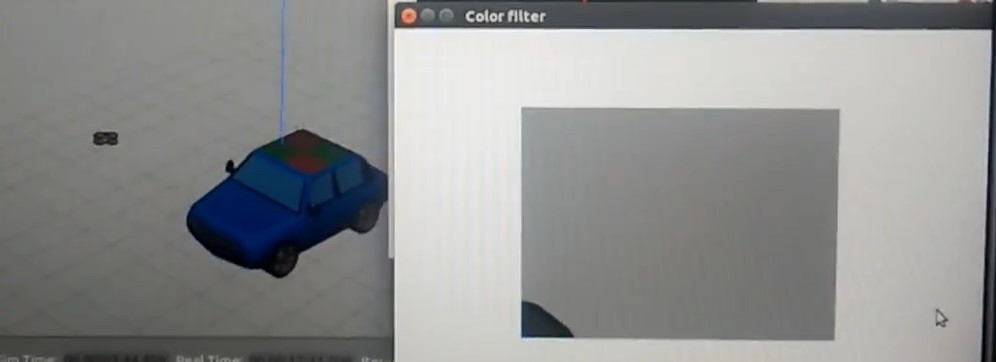
\includegraphics[width=0.33\textwidth]{imgs/busqueda1.jpg}}
  \subfloat[Busqueda]{
   \label{f:Busqueda}
    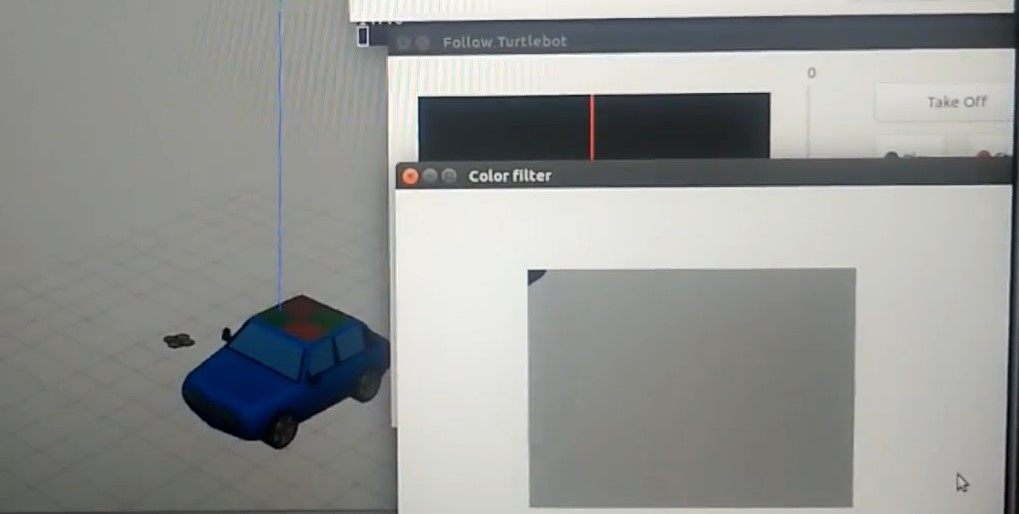
\includegraphics[width=0.33\textwidth]{imgs/busqueda3.jpg}}
	\subfloat[Busqueda]{
   \label{f:Busqueda}
    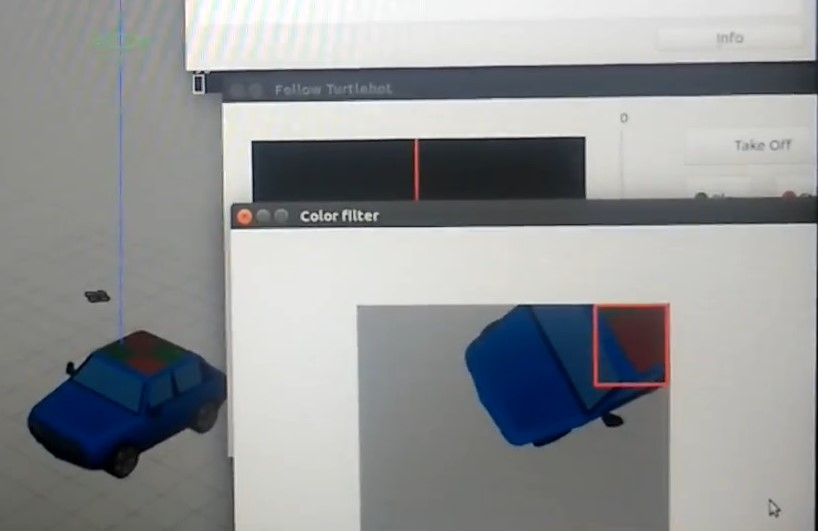
\includegraphics[width=0.33\textwidth]{imgs/busqueda5.jpg}}\\
	\subfloat[Busqueda]{
   \label{f:Busqueda}
    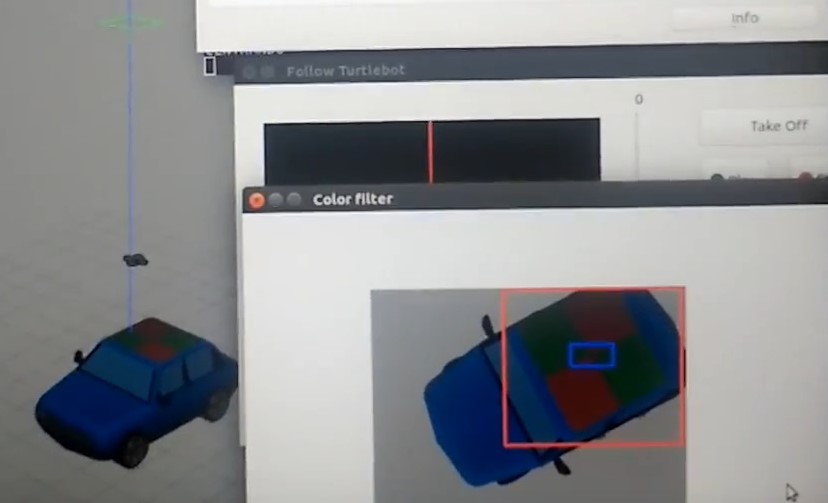
\includegraphics[width=0.4\textwidth]{imgs/busqueda6.jpg}}
	\subfloat[Busqueda]{
   \label{f:Busqueda}
    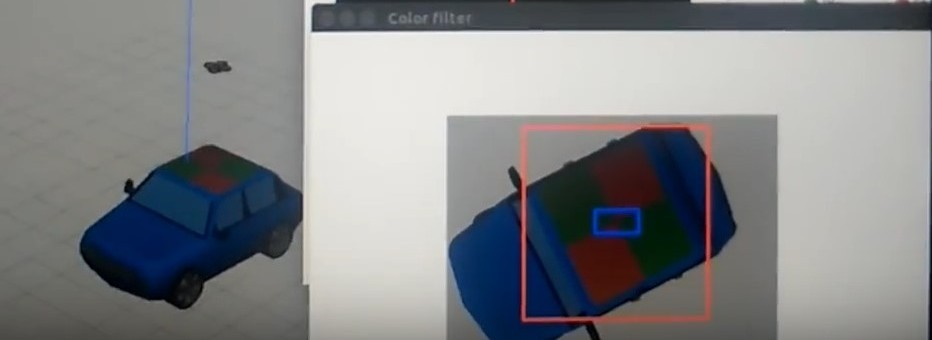
\includegraphics[width=0.4\textwidth]{imgs/busqueda7.jpg}}
 \caption{Busqueda}
 \label{f:Busqueda sobre el simulador}
\end{figure}


\hspace{1cm} Para las pruebas con del drone real, primero se probo solo que el algoritmo de busqueda era correcto, y que el drone realizaba espirales de forma correcta. Pero despues, al realizar las pruebas finales en espacios mas pequeños se modific\'o el algoritmo de b\'usqueda, haciendo que el drone se moviera haciendo cuadrados para tener un mayor control sobre \'este. 

\begin{figure}[H]
 \centering
  \subfloat[Busqueda]{
   \label{f:Busqueda}
    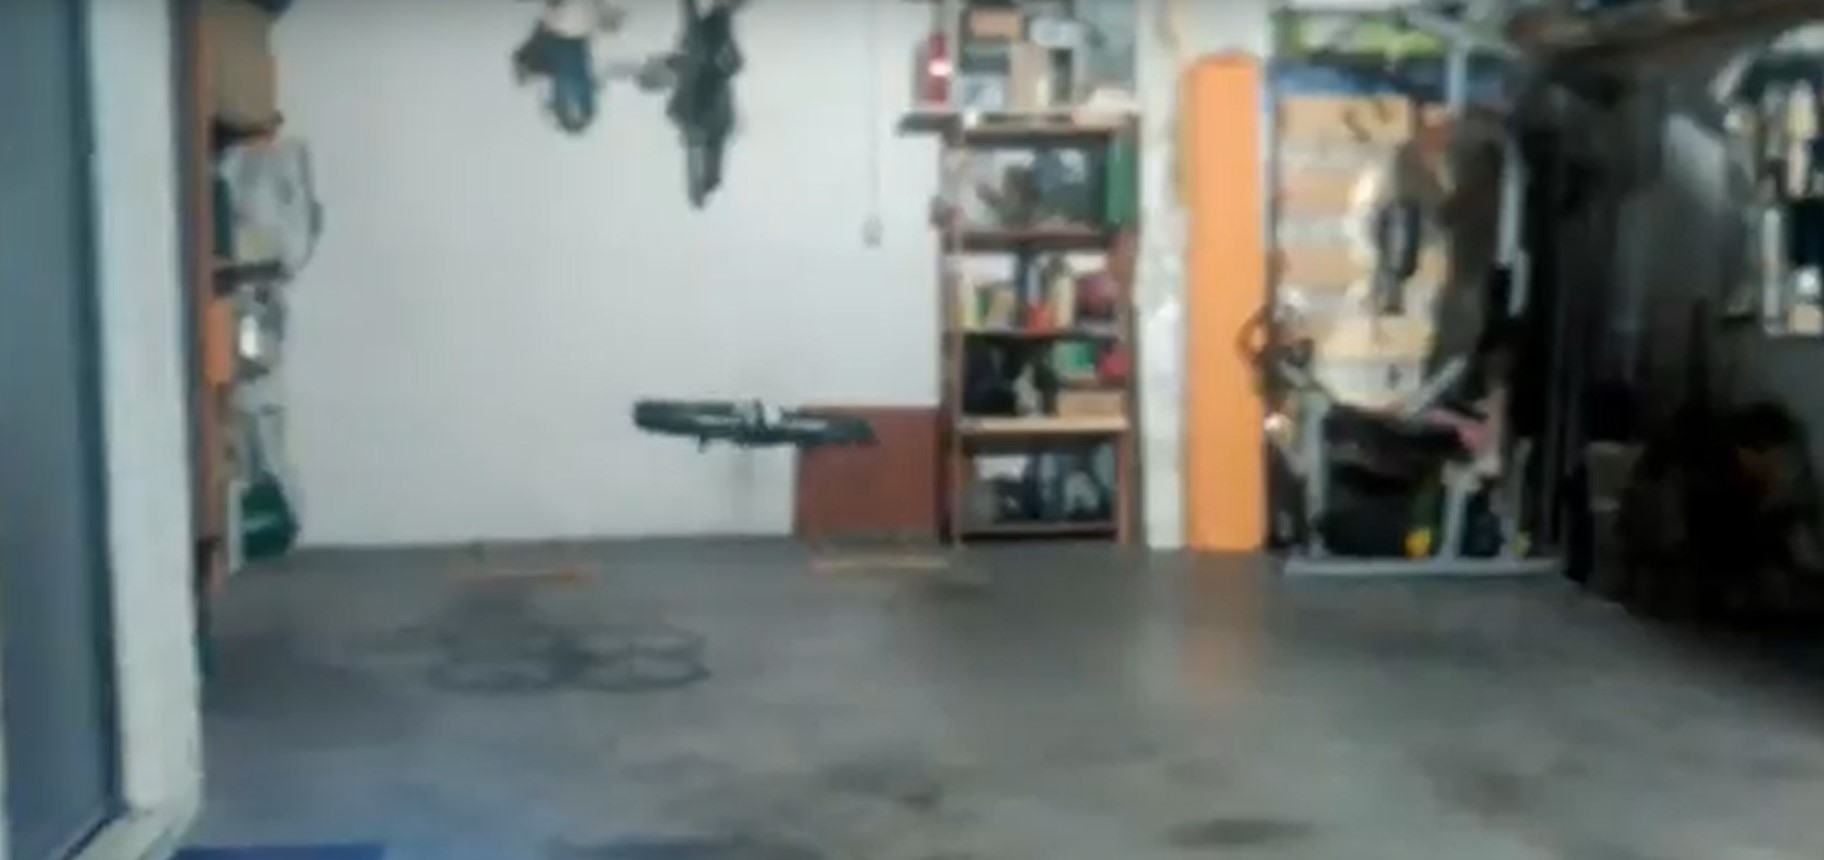
\includegraphics[width=0.33\textwidth]{imgs/busqueda_real1.jpg}}
  \subfloat[Busqueda]{
   \label{f:Busqueda}
    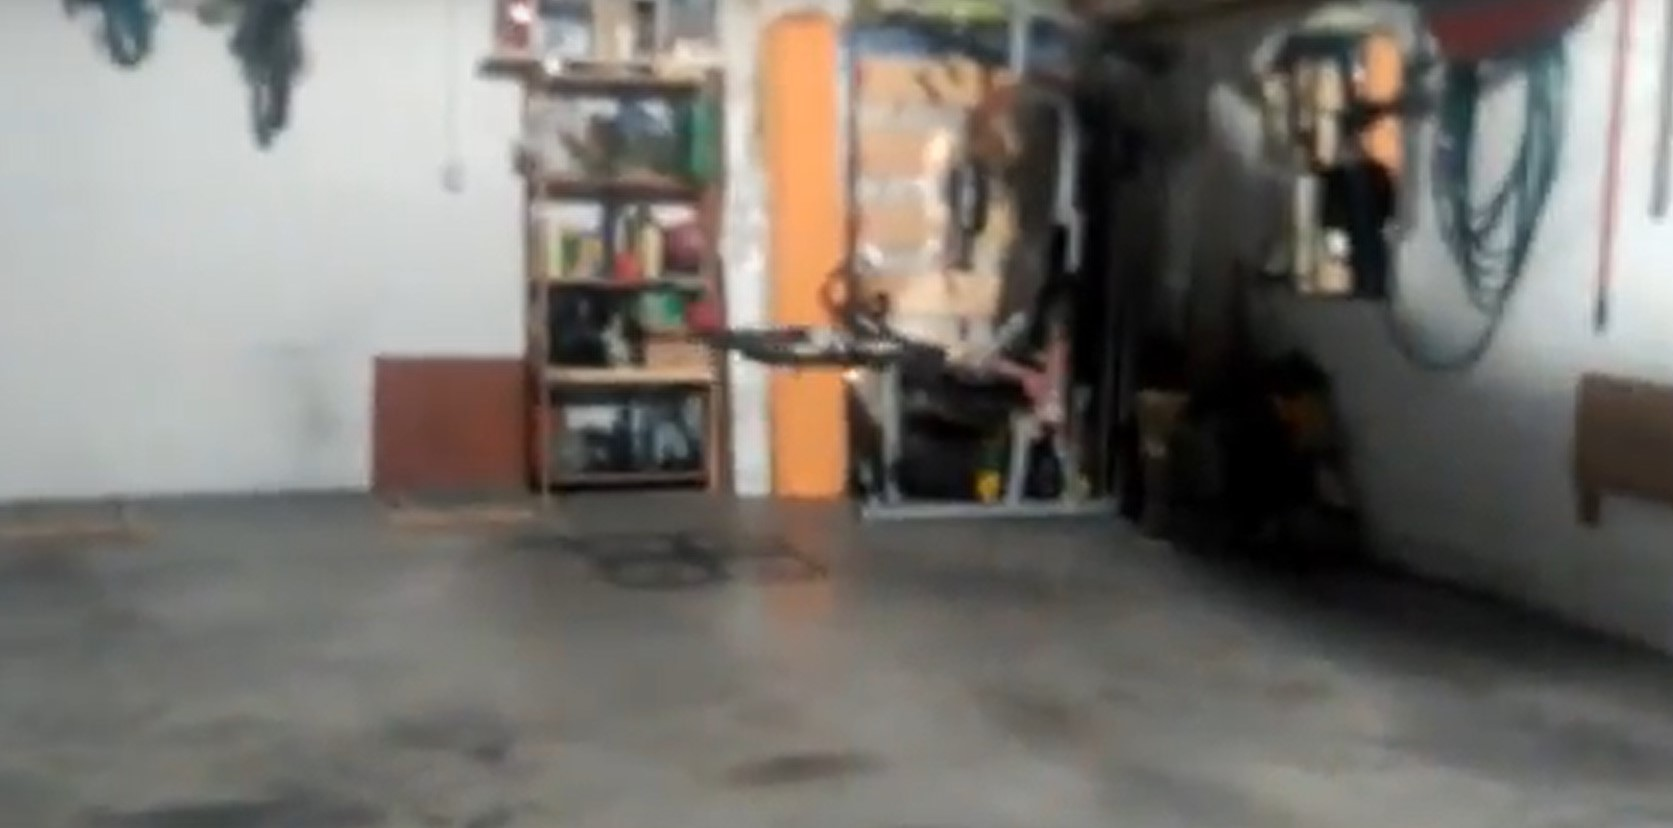
\includegraphics[width=0.33\textwidth]{imgs/busqueda_real3.jpg}}
	\subfloat[Busqueda]{
   \label{f:Busqueda}
    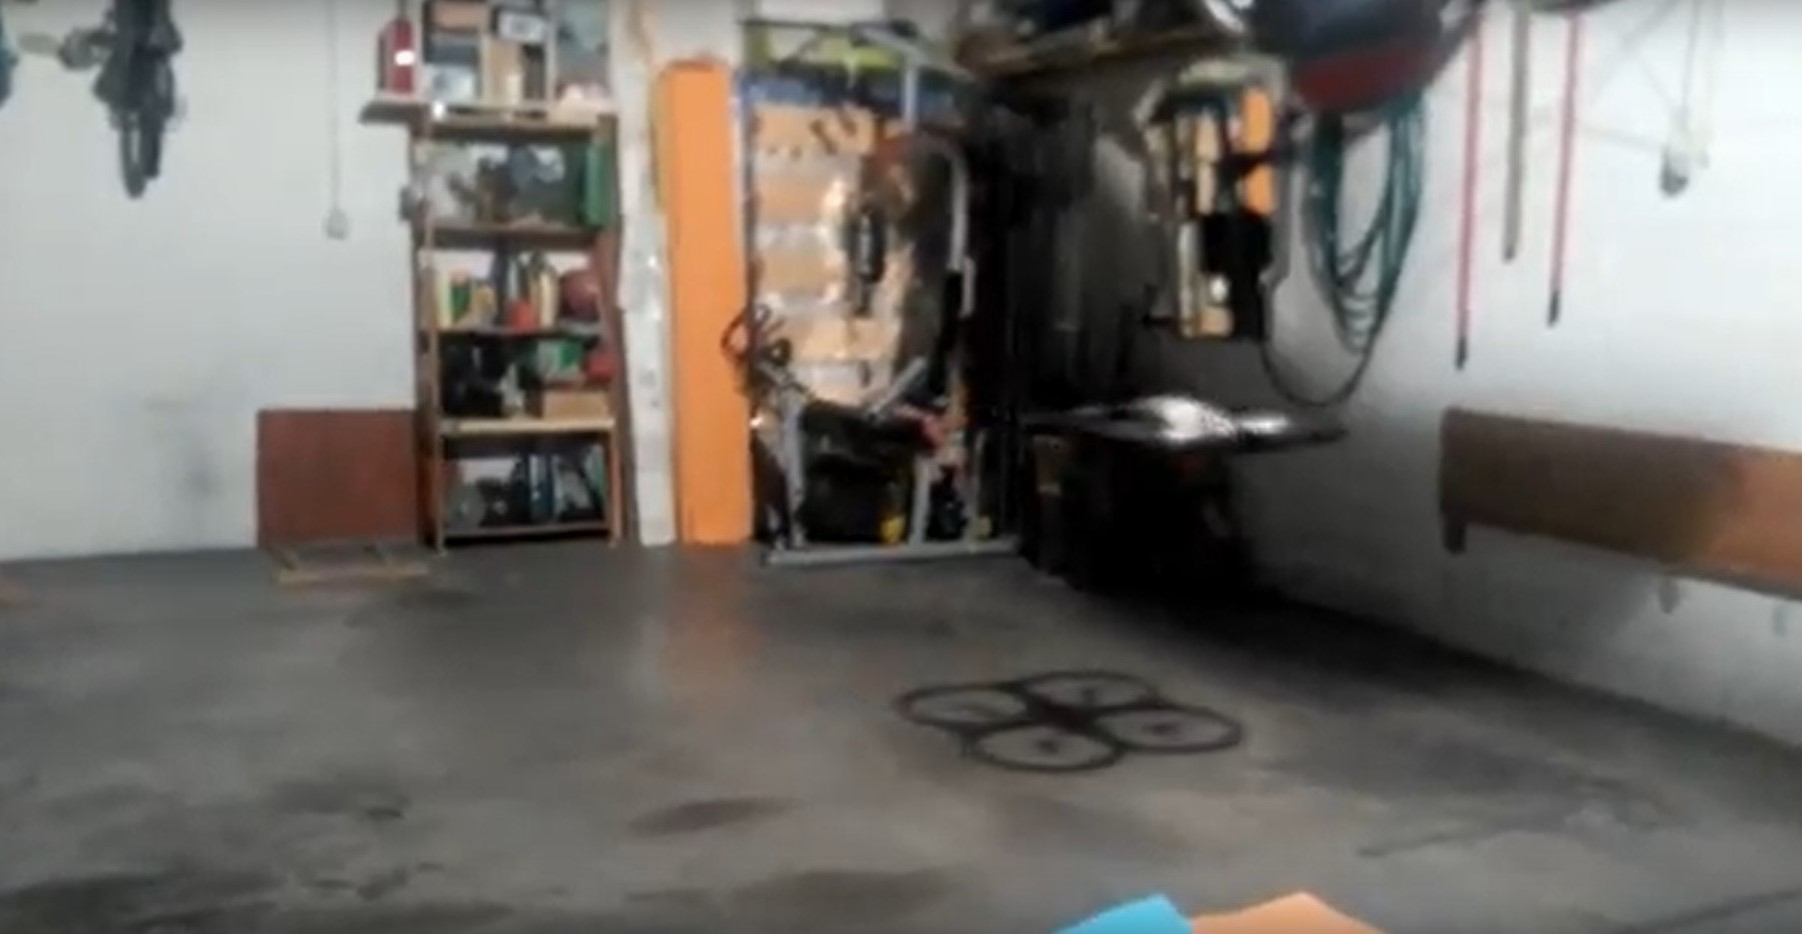
\includegraphics[width=0.33\textwidth]{imgs/busqueda_real5.jpg}}\\
	\subfloat[Busqueda]{
   \label{f:Busqueda}
    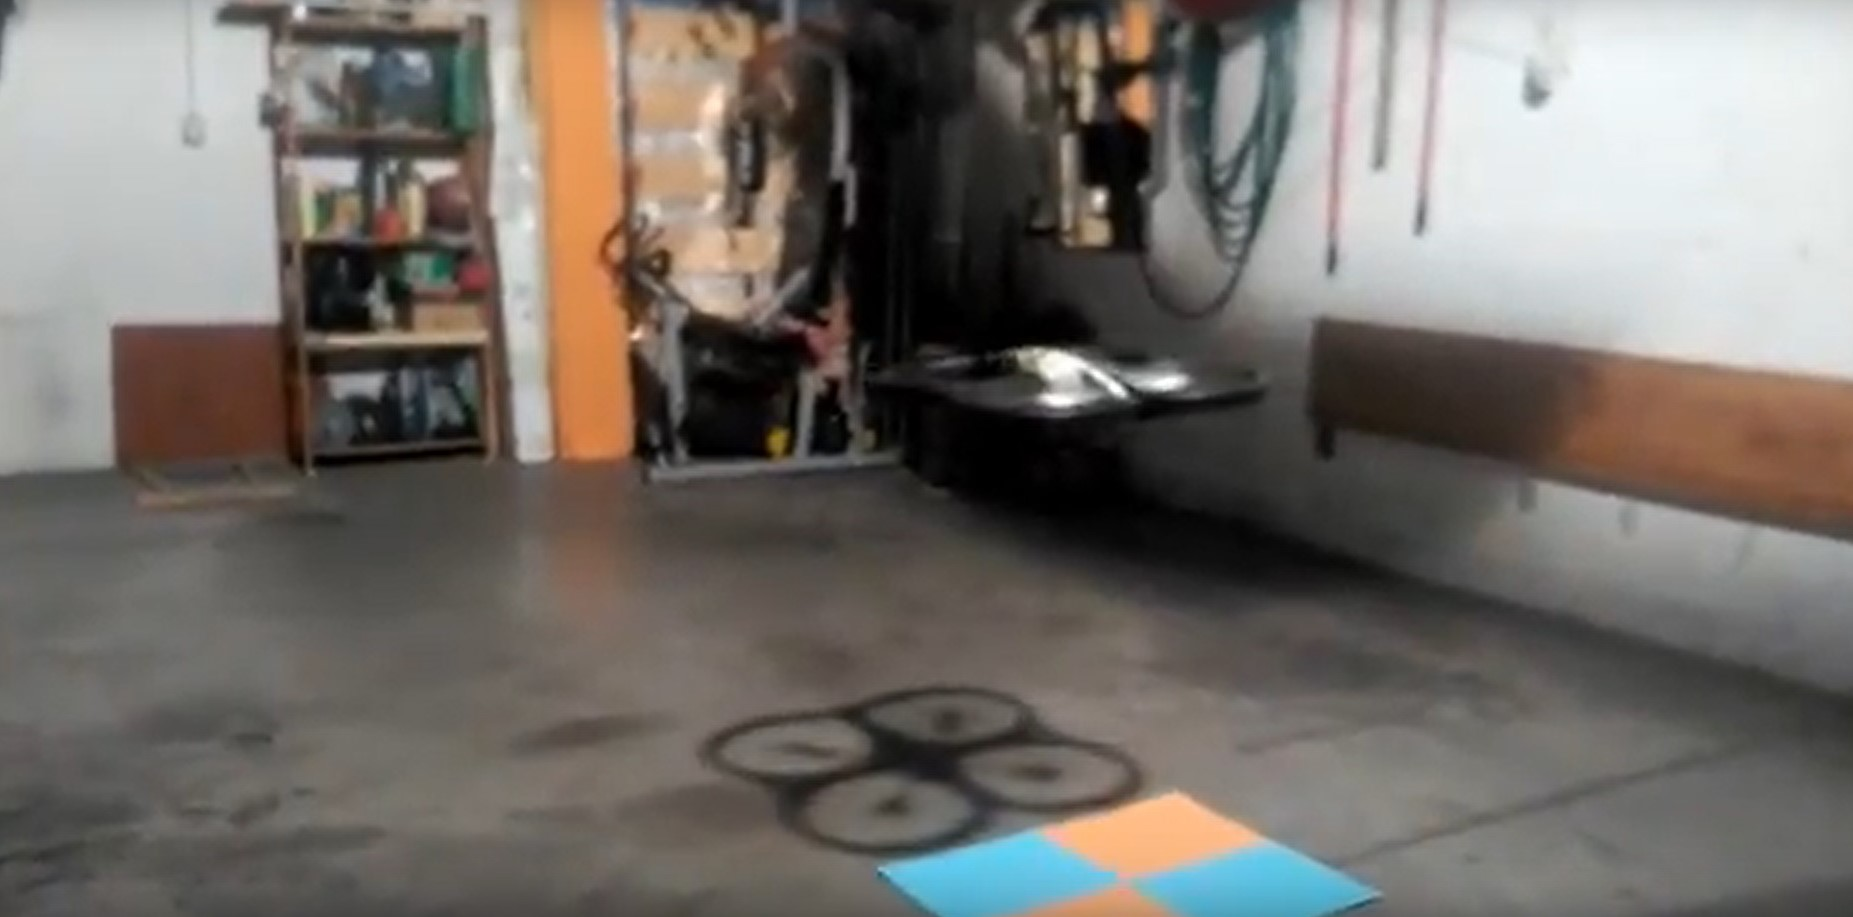
\includegraphics[width=0.4\textwidth]{imgs/busqueda_real6.jpg}}
	\subfloat[Busqueda]{
   \label{f:Busqueda}
    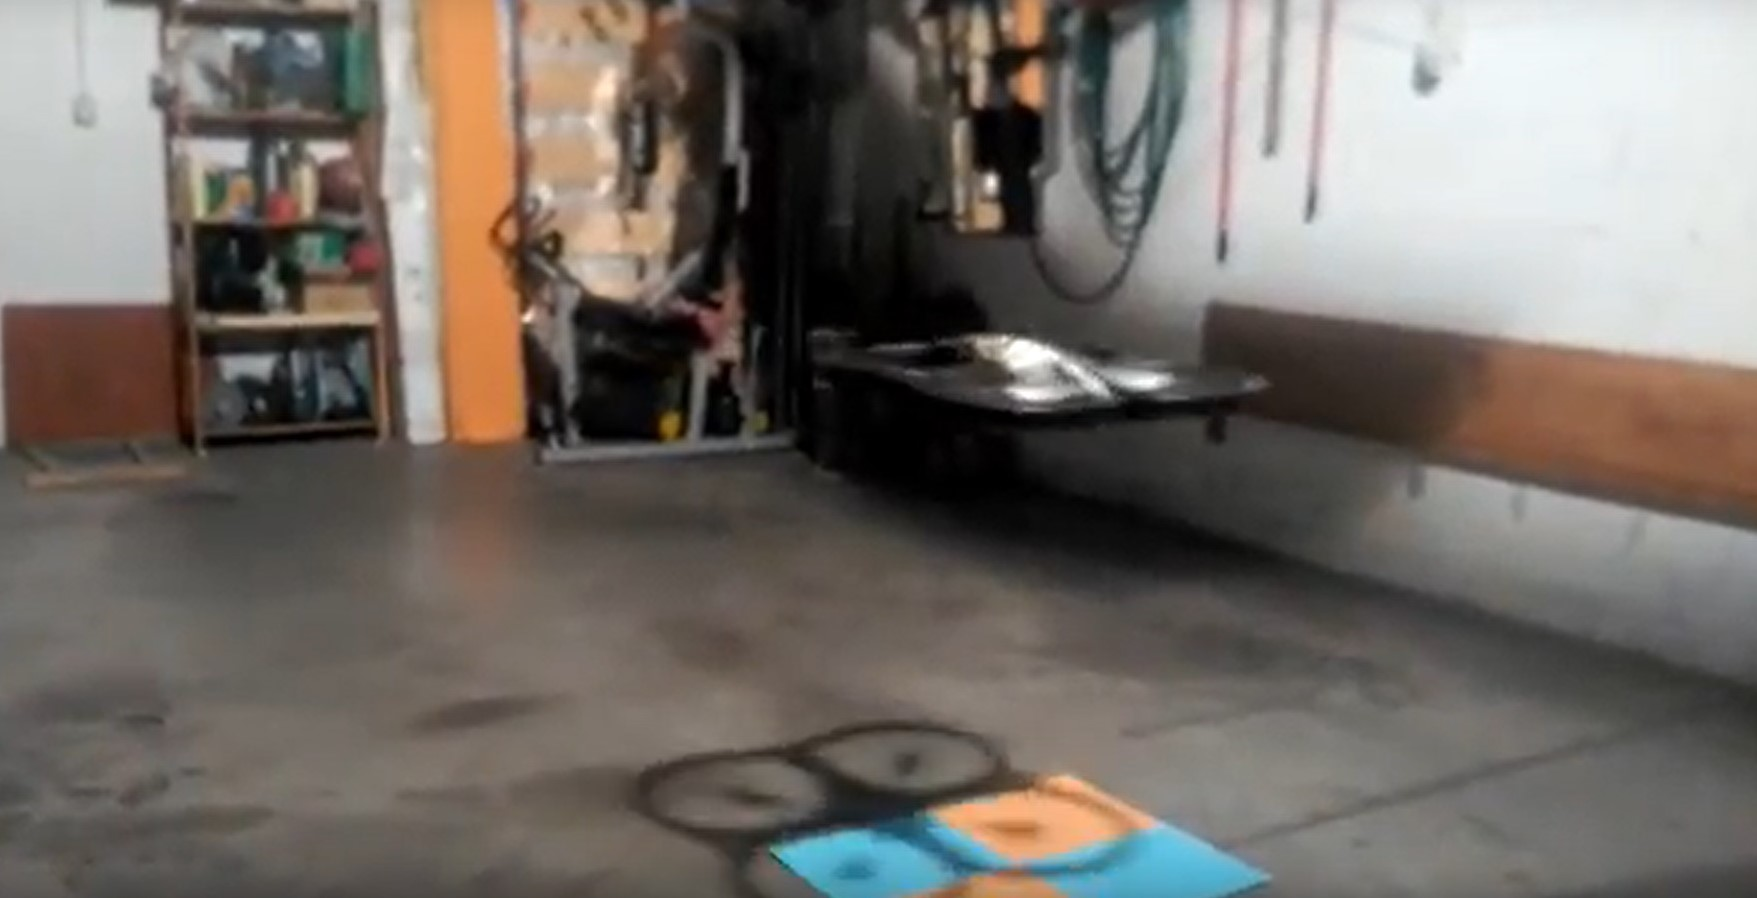
\includegraphics[width=0.4\textwidth]{imgs/busqueda_real7.jpg}}
 \caption{Busqueda}
 \label{f:Busqueda sobre el simulador}
\end{figure}


\section{Aterrizaje. }

\hspace{1cm} En los experimentos de esta parte, lo que se trat\'o fue que el drone se centrara sobre la baliza sin realizar movimientos bruscos, una vez que el drone detectaba que estaba pr\'acticamente centrado sobre la baliza, comenzaba a descender, y una vez detectaba que estaba lo suficientemente cerca enviaba la orden de aterrizar. Como podemos observar, en estos experimentos la parte de percepci\'on se basan en controlar el centro de la baliza y el \'area, para tener una aproximaci\'on de la distancia que hab\'ia a \'esta. 

\begin{figure}[H]
 \centering
  \subfloat[Aterrizaje]{
   \label{f:Aterrizaje}
    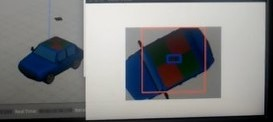
\includegraphics[width=0.33\textwidth]{imgs/landing1.jpg}}
  \subfloat[Aterrizaje]{
   \label{f:Aterrizaje}
    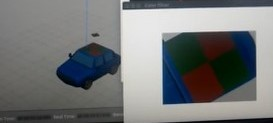
\includegraphics[width=0.38\textwidth]{imgs/landing2.jpg}}
	\subfloat[Aterrizaje]{
   \label{f:Aterrizaje}
    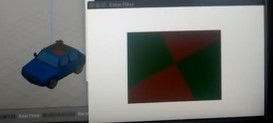
\includegraphics[width=0.33\textwidth]{imgs/landing3.jpg}}\\
	\subfloat[Aterrizaje]{
   \label{f:Aterrizaje}
    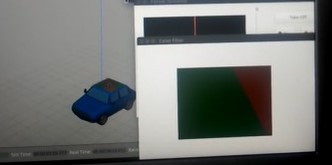
\includegraphics[width=0.4\textwidth]{imgs/landing4.jpg}}
 \caption{Aterrizaje}
 \label{f:Aterrizaje sobre el simulador}
\end{figure}


\hspace{1cm} Para la realizaci\'on de estas pruebas ha habido varias fases. En la primera, cuando el drone estaba en el aire se pon\'ia delante de el la baliza de un color y al detectarla aterrizaba. Una vez funciono esto, se probo poniendo la baliza bajo el mientras no se le mandaban \'ordenes de velocidad, y ya para finalizar que mientras realizaba el algoritmo de b\'usqueda, una vez detectara la baliza aterrizara. Esta prueba los resultados eran buenos, ya que se consegu\'ia que aterrizara, pero por la velocidad que ten\'ia el drone y debido a la inercia, no aterrizaba en el sitio sino que segu\'ia en la misma direcci\'on que ten\'ia anteriormente hasta que se posaba en el suelo y ya se deten\'ia, por lo tanto aterrizaba lejos de la baliza. Pero tras esto y ya añadir los movimientos para centrarse sobre \'esta, se solucion\'o el problema y se consigui\'o que el drone aterrizara verticalmente sobre la baliza. 

\begin{figure}[H]
 \centering
  \subfloat[Aterrizaje]{
   \label{f:Aterrizaje}
    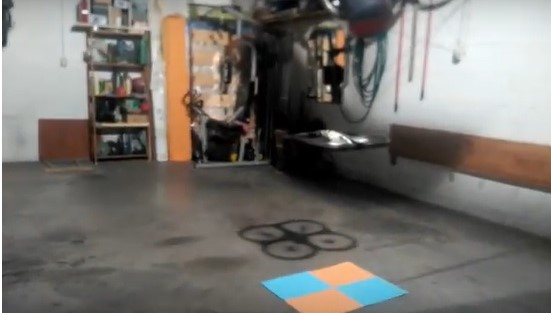
\includegraphics[width=0.33\textwidth]{imgs/aterrizaje_real1.jpg}}
  \subfloat[Aterrizaje]{
   \label{f:Aterrizaje}
    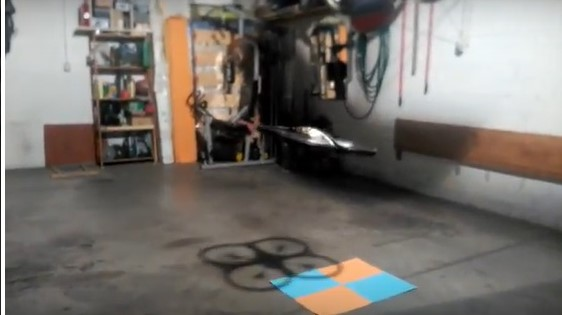
\includegraphics[width=0.33\textwidth]{imgs/aterrizaje_real2.jpg}}
	\subfloat[Aterrizaje]{
   \label{f:Aterrizaje}
    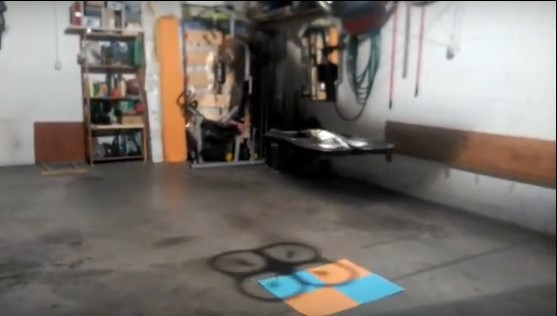
\includegraphics[width=0.33\textwidth]{imgs/aterrizaje_real3.jpg}}\\
	\subfloat[Aterrizaje]{
   \label{f:Aterrizaje}
    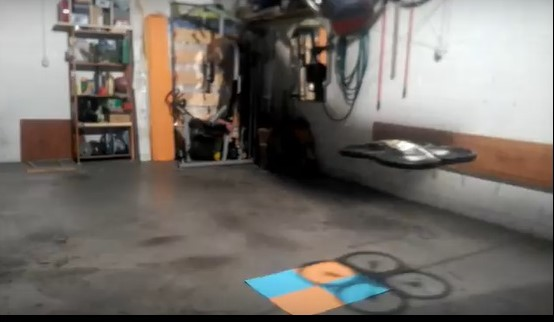
\includegraphics[width=0.33\textwidth]{imgs/aterrizaje_real4.jpg}}
	\subfloat[Aterrizaje]{
   \label{f:Aterrizaje}
    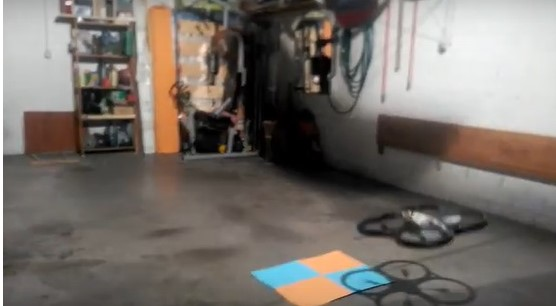
\includegraphics[width=0.33\textwidth]{imgs/aterrizaje_real5.jpg}}
	\subfloat[Aterrizaje]{
   \label{f:Aterrizaje}
    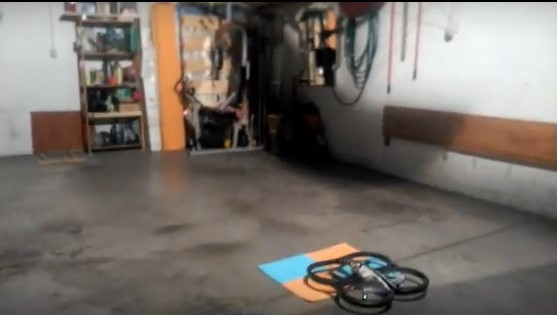
\includegraphics[width=0.33\textwidth]{imgs/aterrizaje_real6.jpg}}
 \caption{Aterrizaje}
 \label{f:Aterrizaje sobre el simulador}
\end{figure}


\section{Algoritmo completo. }
\hspace{1cm} Este experimento se realiz\'o para comprobar que todo lo que se hab\'ia programado por partes funcionaba tambi\'en si se probaba el algoritmo completo. Cabe destacar que las pruebas salieron correctamente. Sobre el simulador se prob\'o a poner el drone sobre la baliza, que despegaba y se situaba en el centro de esta. Una vez pasaron 10 segundos y el drone continuaba en el centro, se hizo que este se alejara y perdiera la referencia de la baliza, y comenzara su algoritmo de b\'usqueda. Una vez realizaba las espirales, en el momento que detectaba los colores de la baliza se centraba sobre estos, y una vez estaba pr\'acticamente centrado, comenzaba a descender, hasta que detectaba que estaba a una altura suficiente y se le pod\'ia mandar la orden de aterrizar, pos\'andose as\'i sobre la baliza. 

A continuaci\'on esta la secuencia de im\'agenes de esta prueba, pero la referencia para con el v\'	ideo es la siguiente:\\
\underline{\url{https://www.youtube.com/watch?time_continue=129&v=g9ZGJhRWTiY}}

\begin{figure}[H]
 \centering
  \subfloat[Despegue]{
   \label{f:Despegue}
    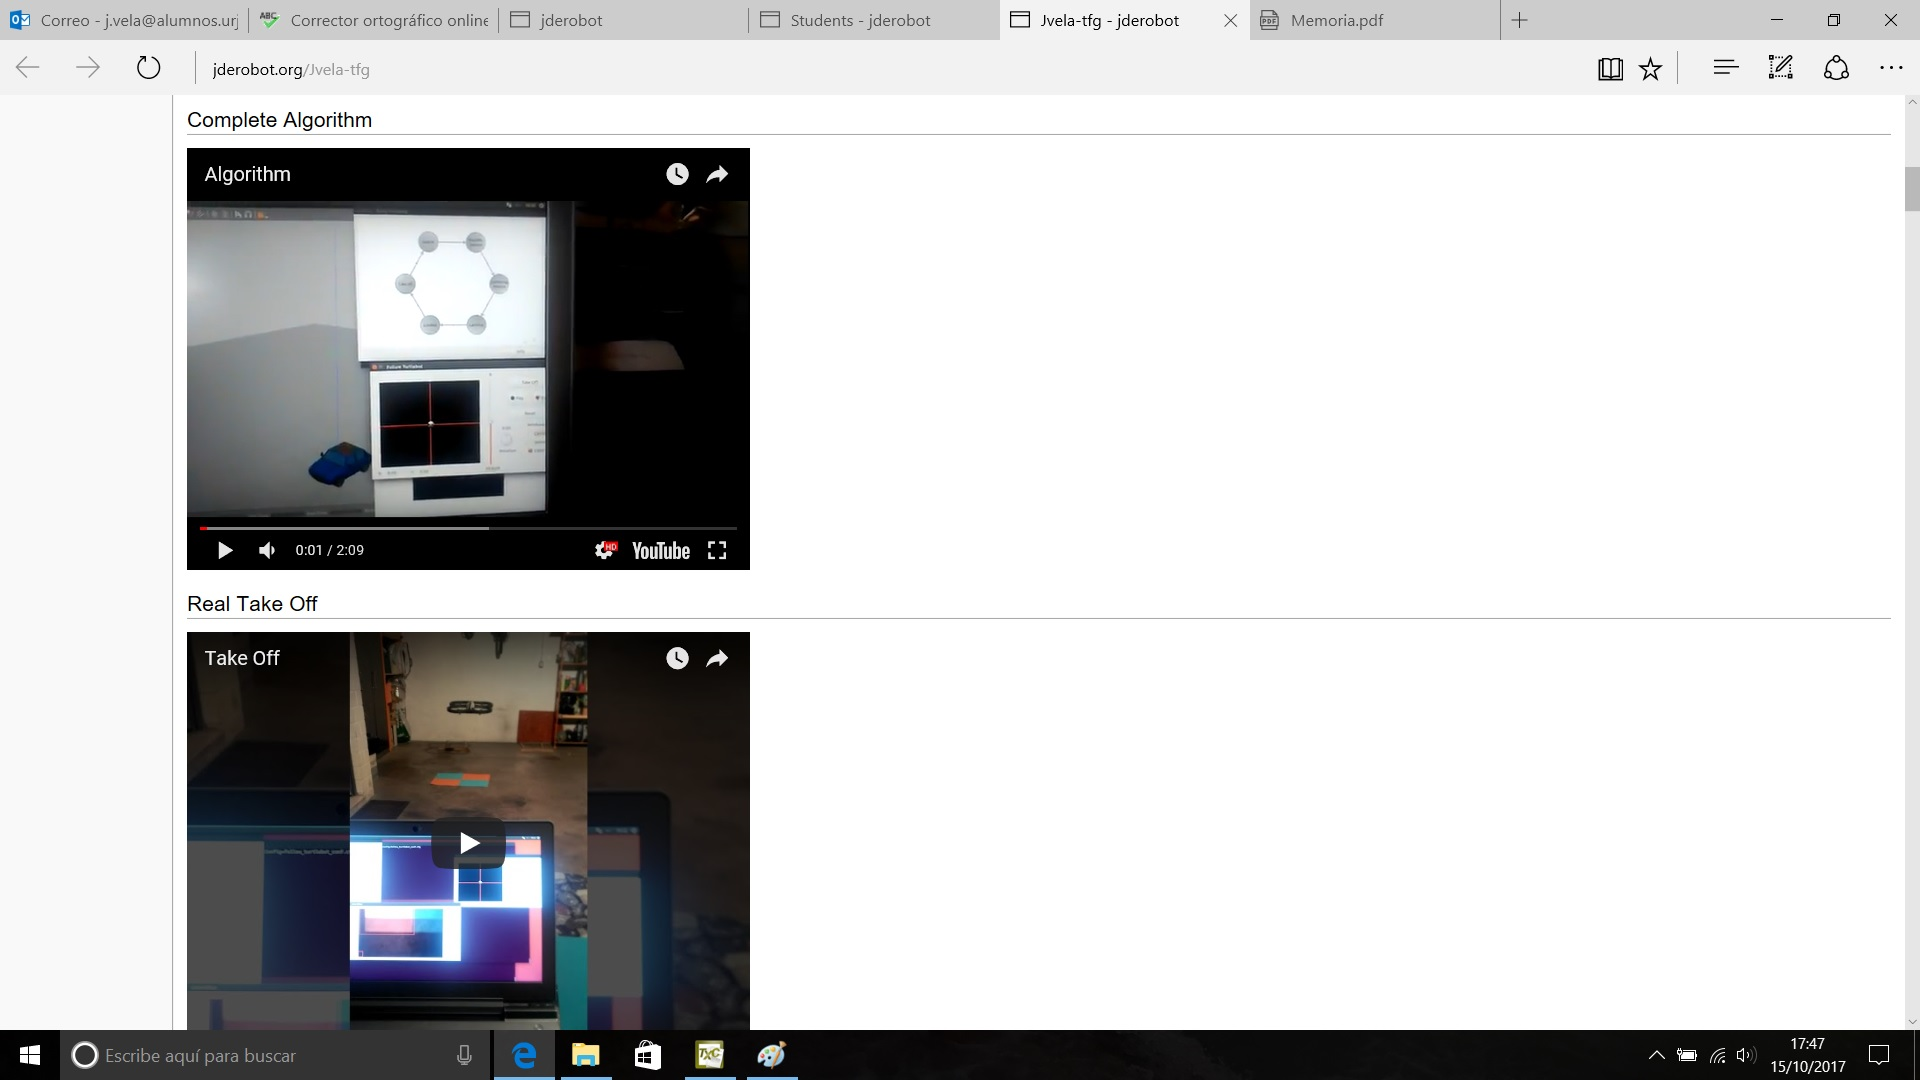
\includegraphics[width=0.25\textwidth]{imgs/total1.jpg}}
  \subfloat[Despegue]{
   \label{f:Despegue}
    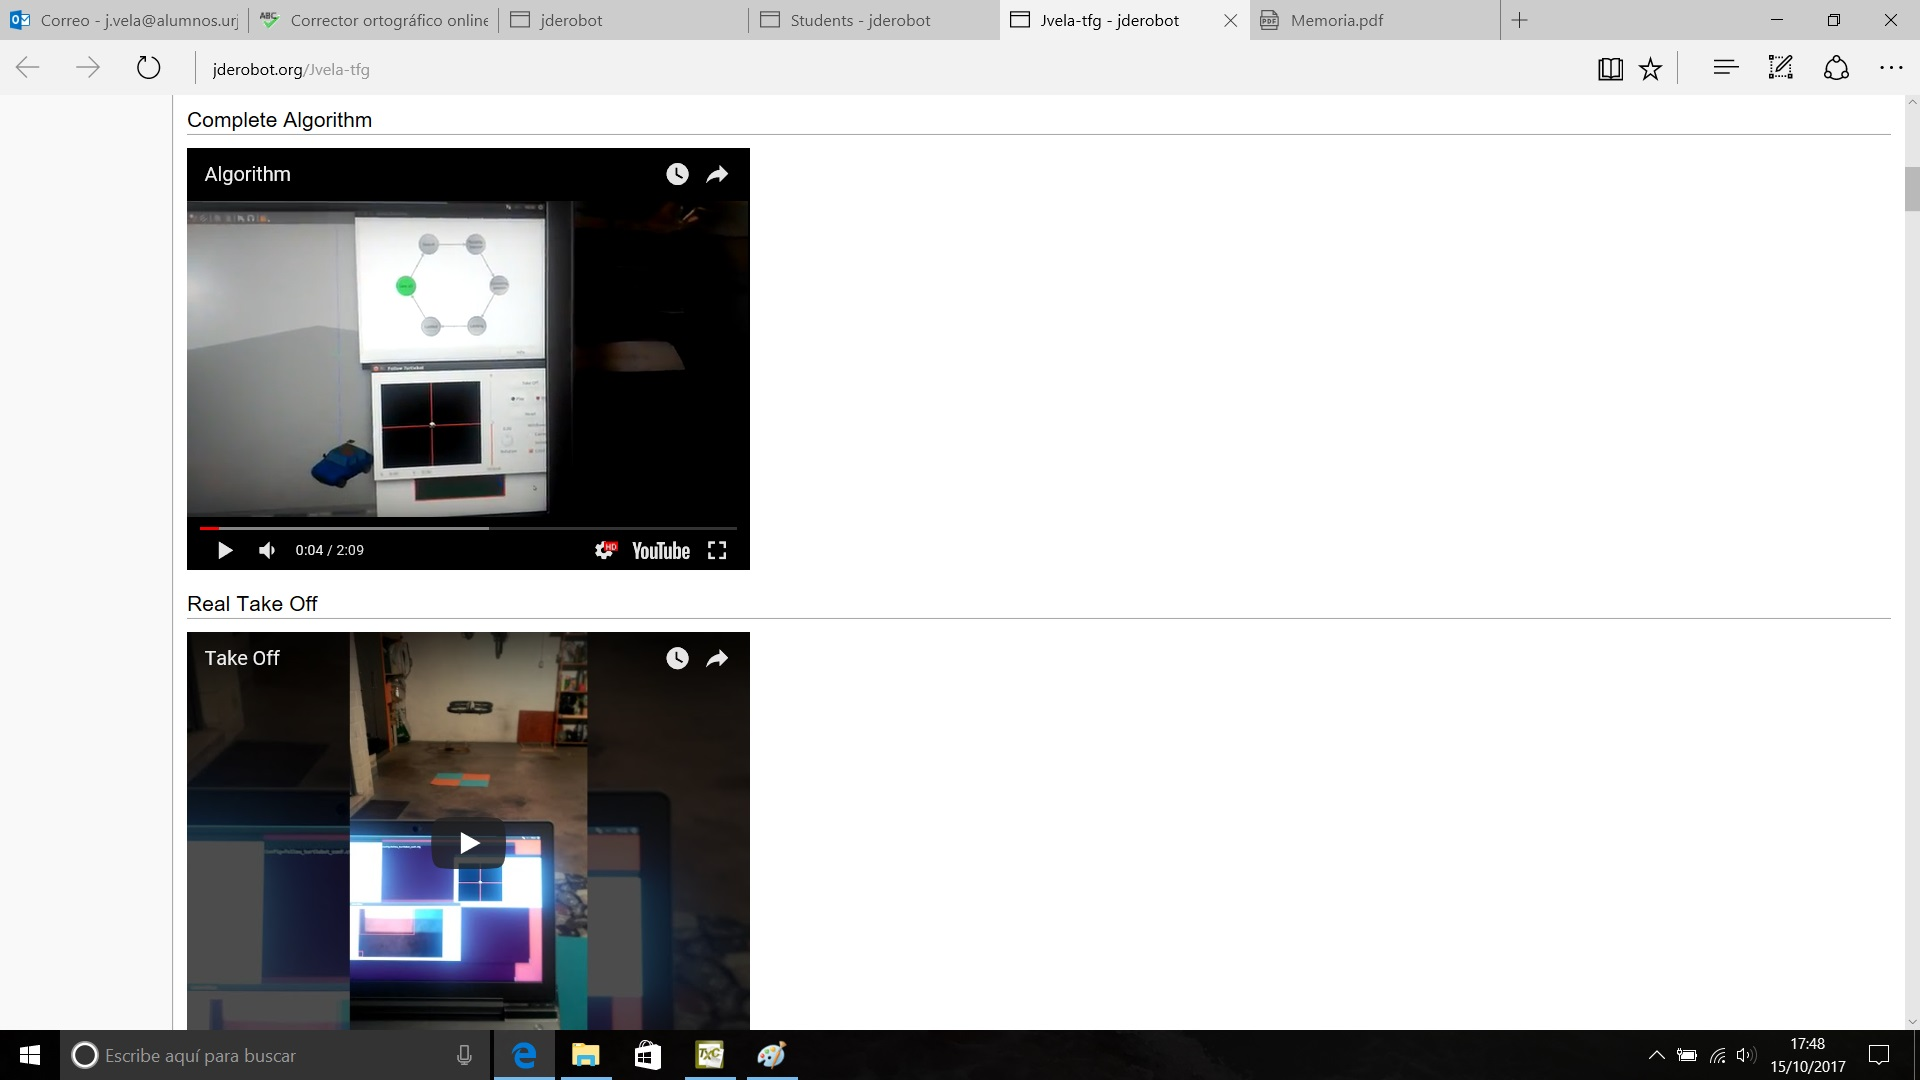
\includegraphics[width=0.25\textwidth]{imgs/total2.jpg}}
	\subfloat[Despegue]{
   \label{f:Despegue}
    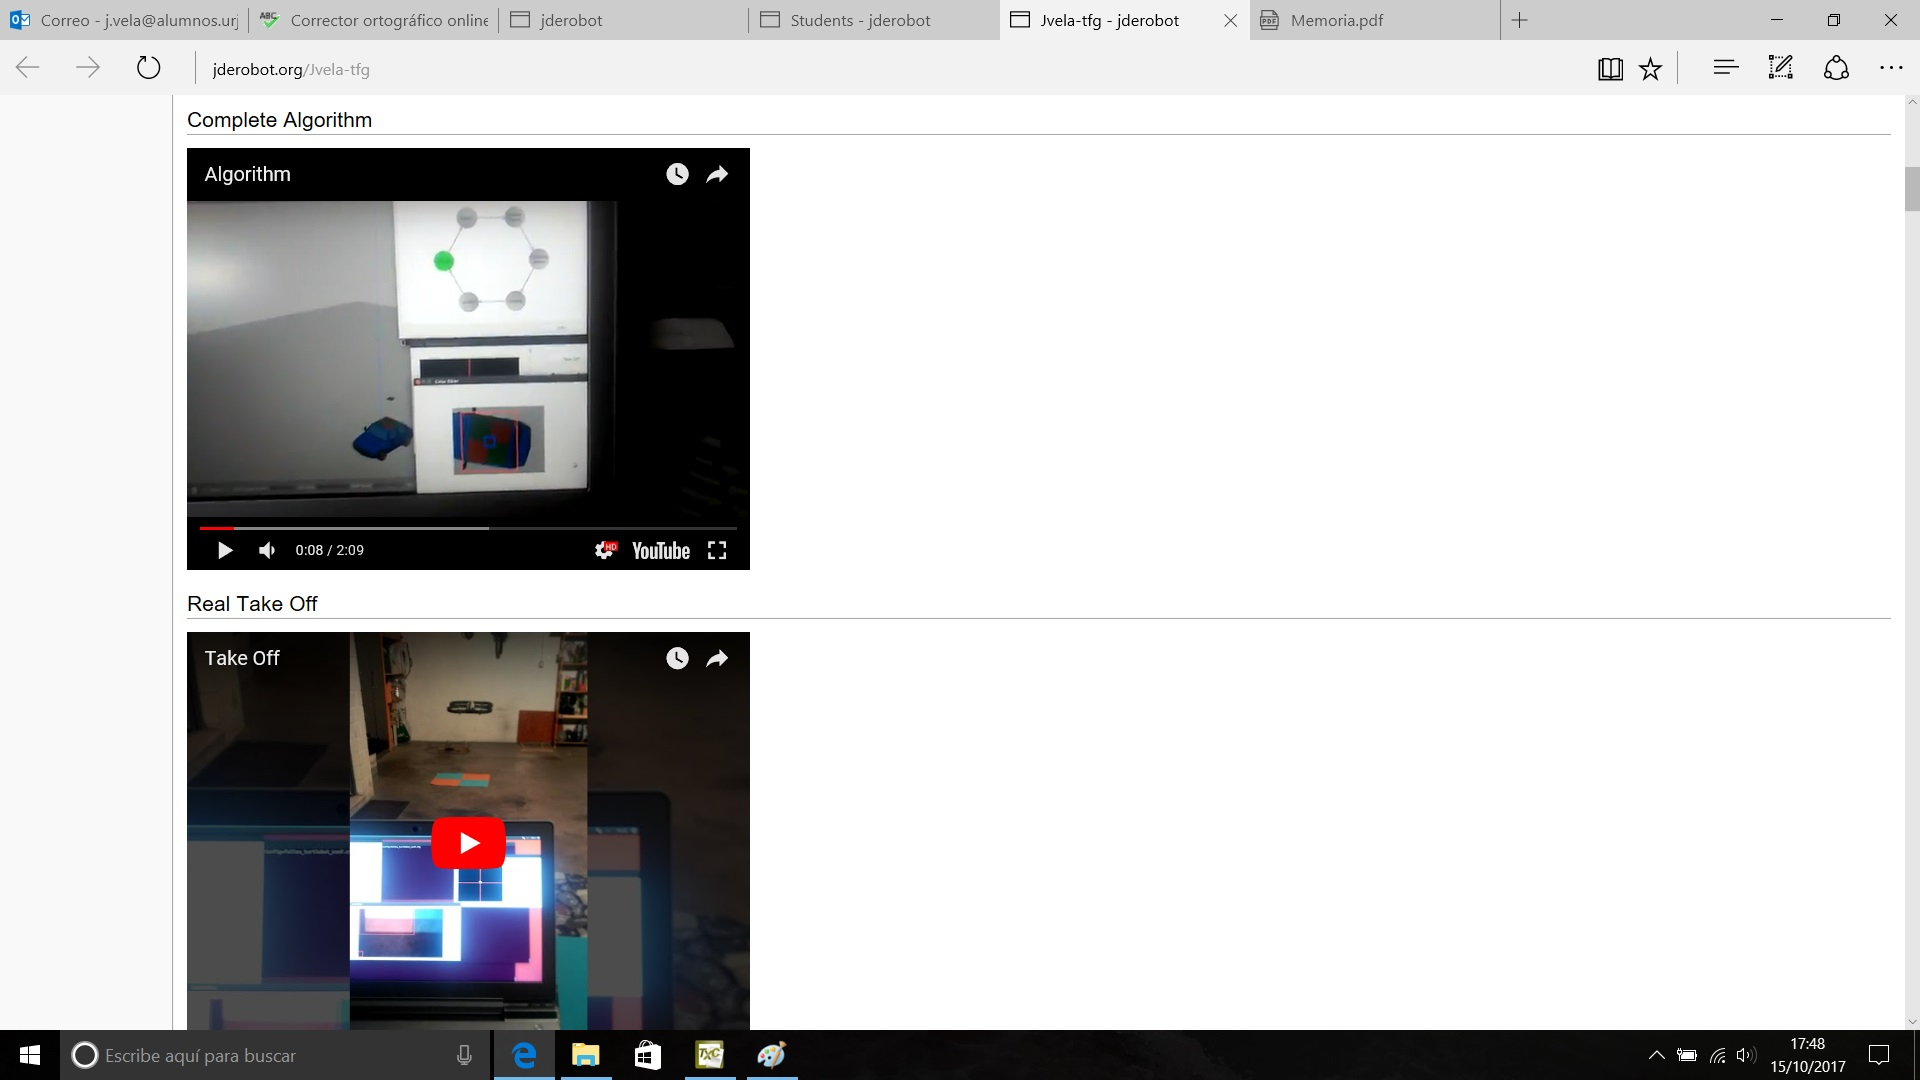
\includegraphics[width=0.25\textwidth]{imgs/total3.jpg}}
	\subfloat[Despegue]{
   \label{f:Despegue}
    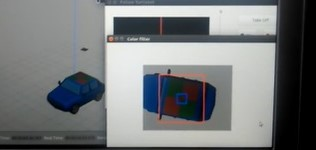
\includegraphics[width=0.25\textwidth]{imgs/total4.jpg}}\\
	\subfloat[Alejandose de la baliza]{
   \label{f:Alejandose de la baliza}
    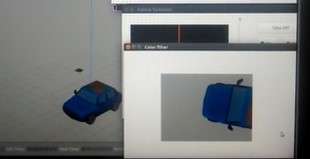
\includegraphics[width=0.25\textwidth]{imgs/total5.jpg}}
	\subfloat[Busqueda]{
   \label{f:Busqueda}
    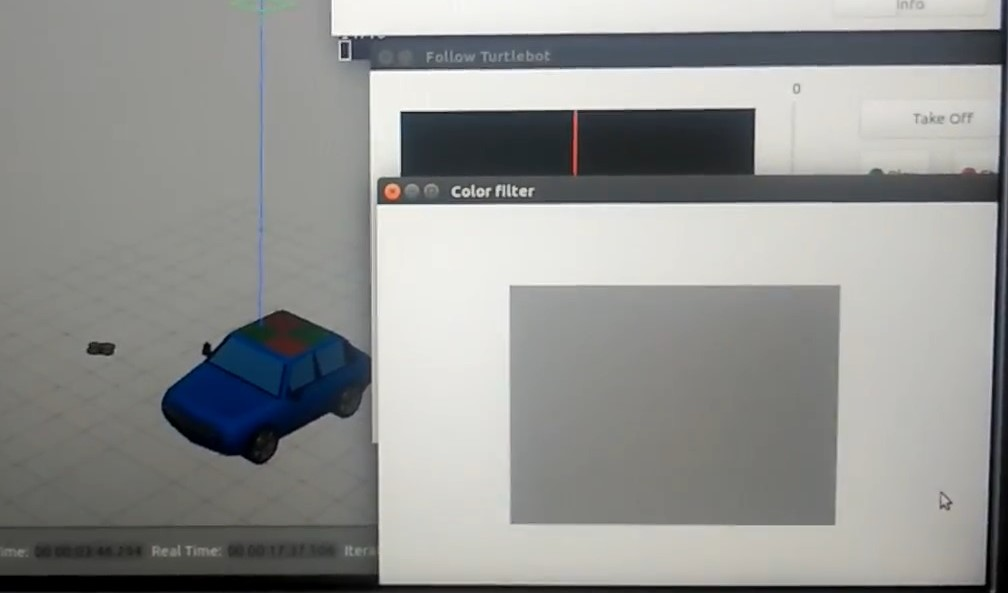
\includegraphics[width=0.25\textwidth]{imgs/busqueda2.jpg}}
	\subfloat[Busqueda]{
   \label{f:Busqueda}
    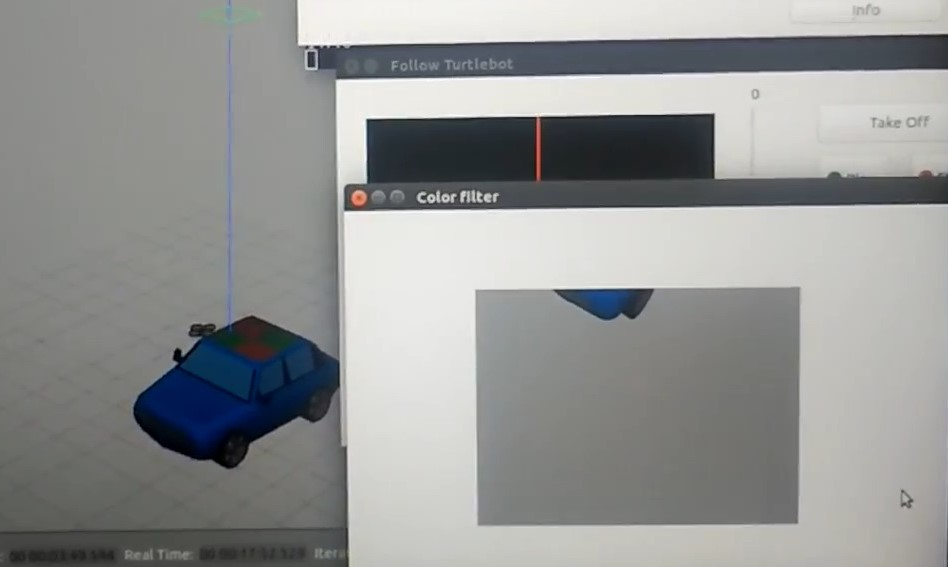
\includegraphics[width=0.25\textwidth]{imgs/busqueda4.jpg}}
	\subfloat[Busqueda]{
   \label{f:Busqueda}
    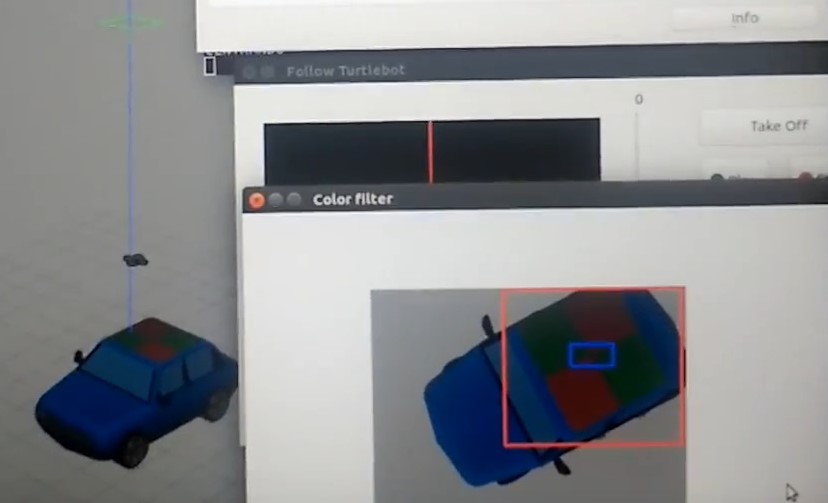
\includegraphics[width=0.25\textwidth]{imgs/busqueda6.jpg}} \\
		  \subfloat[Aterrizaje]{
   \label{f:Aterrizaje}
    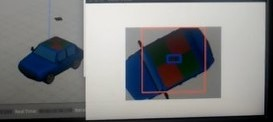
\includegraphics[width=0.25\textwidth]{imgs/landing1.jpg}}
  \subfloat[Aterrizaje]{
   \label{f:Aterrizaje}
    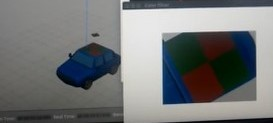
\includegraphics[width=0.30\textwidth]{imgs/landing2.jpg}}
	\subfloat[Aterrizaje]{
   \label{f:Aterrizaje}
    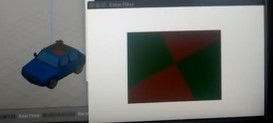
\includegraphics[width=0.25\textwidth]{imgs/landing3.jpg}}
	\subfloat[Aterrizaje]{
   \label{f:Aterrizaje}
    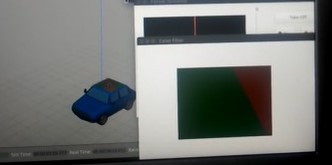
\includegraphics[width=0.25\textwidth]{imgs/landing4.jpg}}
 \caption{Algoritmo completo sobre el simulador. }
 \label{f:Algoritmo completo sobre el simulador. }
\end{figure}


\hspace{1cm} Para la prueba con el drone real se colocaron dos puntos de referencia. Una baliza sobre la que situarse al despegar. De esta forma al comenzar el algoritmo, cuando detectaba esta baliza se centraba sobre \'esta, y una vez pasaron 10 segundos comenzaba el algoritmo de b\'usqueda. En esta parte el drone se iba desplazando en funci\'on de las ordenes que se le mandaban en cada momento, hasta el momento en el que encontraba la baliza, momento en el que se centraba sobre esta y se le mandaba la orden de aterrizaje, quedando de esta forma el drone sobre la baliza. 
